\newpage
\section{Part 4: Expectation Maximization (EM)}
\label{sec:em}

In section \ref{sec:baumwelch} we have seen how the Baum-Welch algorithm progressively refines the estimation of model parameters $\theta$, improving their likelihood estimate. In this section we will see how this notion can be generalized to an algorithm that aims to improve the likelihood of model parameters iteratively, especially in situations where such estimation relies on {\bf unobserved hidden variables} or {\bf missing data} $m$.
This algorithm is called Expectation Maximization (EM).

EM is about trying to fill in the missing variables $m$ using a probabilistic model. It can be applied to any probababilistic model, such as bayesian networks   or graphical models, and there is indeed a lot of scientific literature about applying EM algorithms to various models.
 
The goal of the EM algorithm is to optimize the likelihood of the parameters $\theta$: start from $\theta_0$, improve its likelihood successively until an optimum $\theta^{*}$ is reached:
\begin{equation}
\theta_0  \rightarrow \theta_1 \rightarrow ... 
\rightarrow \theta_i, \rightarrow \theta_{i+1}
\rightarrow ... \rightarrow \theta^{*} 
\end{equation}

At each step, the change in $\Delta(\theta_{i+1}, \theta_i)$ in log-likelihood is measured:
\begin{equation}
\Delta(\theta_{i+1}, \theta_i) 
= \ln \; P(D|\theta_{i+1}) - \ln P(D|\theta_i)
= \ln \; \frac{P(D|\theta_{i+1})}{P(D|\theta_i)}
\end{equation}

Optimizing the likelihood then amounts to keeping $\Delta(\theta_{i+1}, \theta_i)$ positive. However the missing data $m$ complicates the computation of the likelihood: instead of having $P(D|\theta)$, usually what we have is $P(D,m|\theta)$. The usual way to deal with $m$ is via marginalization:
%
\begin{itemize}
\item If $m$ is discrete:
\begin{equation}
P(D|\theta) = E_{m|\theta}[P(D,m|\theta)] = \sum_m P(D,m|\theta) = 
\sum_m P(D|m,\theta) P(m|\theta)
\end{equation}
%
\item If $m$ is continuous:
\begin{equation}
P(D|\theta) = E_{m|\theta}[P(D,m|\theta)] = \int_m P(D,m|\theta) dm = 
\int_m P(D|m,\theta) P(m|\theta) dm
\end{equation}
\end{itemize}
%
where $E_{m|\theta}[P(D,m|\theta)]$ is the {\bf expectation} of $P(D,m|\theta)$ over all possible values of $m$. Note that this is the same as what was done in the forward algorithm where $D$ was the sequence $x$ and $m$ was the path $\pi$.

We'll assume that $m$ is discrete from now on for simplification. 
%\textcolor{red}{Moreover we'll use the values of $m$ estimated in the present iteration as input for the next iteration, so we consider for simplification that $m$ is only missing at the next iteration????} 
The measurement of likelihood improvement then becomes:
\begin{eqnarray}
\Delta(\theta_{i+1}, \theta_i) & = &
\ln E[P(D,m|\theta_{i+1})] - \ln P(D|\theta_i) \\ & = &
\ln \frac{\sum_m P(D,m|\theta_{i+1})}{ P(D|\theta_i) } =
\ln \sum_m \frac{P(D,m|\theta_{i+1})}{ P(D|\theta_i) }
\label{eq:em:logsum}
\end{eqnarray}

Note that only the term for iteration $i+1$ is marginalizing the missing variables $m$. Moreover since the denominator is not dependent on $m$, it is ok to push it inside the sum.
Anyway the solution of eq. (\ref{eq:em:logsum}) turns out to be difficult mathematically because of the log of a sum.
%
The technique is to use {\bf Jensen's inequality} to get a lower bound $\delta$ on $\Delta$. %(\theta_{i+1}, \theta_i)
If $\delta > 0$ at each iteration, then we're sure that $\Delta > 0$ too, by only measuring $\delta$.

Jensen's inequality guarantees that the log of a sum is always larger than a weighted sum of logs, for positive weights $\lambda_j$ that sum up to one:
\begin{equation}
\ln \sum_j \lambda_j y_j \ge \sum \lambda_j \ln y_j 
\quad \text{for} \quad \lambda_j > 0 \; \text{and} \; \sum_j \lambda_j = 1
\end{equation}

%the variation $\Delta$ of the likelihood from $\theta_i$ to $\theta_{i+1}$:
Let's multiply eq. (\ref{eq:em:logsum}) by $\lambda_m = P(m|D,\theta_i)$ up and down such that it doesn't change:
\begin{eqnarray}
\Delta(\theta_{i+1}, \theta_i) & = &
\ln \sum_m \frac{P(D,m|\theta_{i+1}) P(m|D,\theta_i)}
                { P(D|\theta_i) P(m|D,\theta_i)}
\\
& = &
\ln \sum_m P(m|D,\theta_i) \frac{P(D,m|\theta_{i+1}) }{ P(D,m|\theta_i)}
\label{eq:em:logsum2}
\end{eqnarray}

Now choose $\lambda_m = P(m|D,\theta_i)$ and $y_m = \frac{P(D,m|\theta_{i+1}) }{ P(D,m|\theta_i)}$ in order to apply Jensen's inequality:

\begin{eqnarray}
\Delta(\theta_{i+1}, \theta_i) & = &
\ln \sum_m P(m|D,\theta_i) \frac{P(D,m|\theta_{i+1}) }{ P(D,m|\theta_i)}
\\
& = &
\ln \sum_m \lambda_m y_m \ge 
\sum_m \lambda_m \ln y_m 
\\
& = &
\sum_m P(m|D,\theta_i) \ln \frac{P(D,m|\theta_{i+1}) }{ P(D,m|\theta_i)}
\\
& = &
\delta(\theta_{i+1}, \theta_i)
\label{eq:em:logsum3}
\end{eqnarray}

Now instead of trying to maximize $\Delta$ directly, we maximize $\delta$, the lower bound on the variation in likelihood:
\begin{equation}
\delta(\theta_{i+1}, \theta_i) = \sum_m P(m|D, \theta_i) \; 
                           \ln \frac{P(D,m|\theta_{i+1})}{P(D,m|\theta_i)}
\label{eq:deltaEM}
\end{equation}

The goal of the iterative algorithm is to find the parameters $\theta_{i+1}$ for the next iteration, given the current $\theta_i$, in such a way that $\delta$ is maximized:
\begin{eqnarray}
\theta_{i+1}^{EM} & = & 
     \argmax_\theta \; \delta(\theta, \theta_i^{EM}) \nonumber \\
     & = & \argmax_\theta \; \sum_m P(m|D, \theta_i^{EM}) \; 
                           \ln \frac{P(D,m|\theta)}{P(D,m|\theta_i^{EM})}
\\
     & = & \argmax_\theta \; \sum_m P(m|D, \theta_i^{EM}) \; 
                           ( \ln P(D,m|\theta) - \ln P(D,m|\theta_i^{EM} ) )
\\
     & = & \argmax_\theta \; 
\sum_m P(m|D, \theta_i^{EM}) \ln P(D,m|\theta) 
\nonumber \\
&& \quad \quad \quad 
- \sum_m P(m|D, \theta_i^{EM}) \ln P(D,m|\theta_i^{EM})
\label{eq:em:argmax}
\end{eqnarray}
The superscript EM simply means that these are the optimum parameters chosen by the EM algorithm at each iteration.

The last term of eq. (\ref{eq:em:argmax}) is independent of $\theta$ so it has no influence on the maximum and can be eliminated:
\begin{eqnarray}
\theta_{i+1}^{EM} & = & 
   \argmax_\theta \; \sum_m P(m|D, \theta_i^{EM}) \; 
   \ln \; P(D,m|\theta) \nonumber \\
& = &
   \argmax_\theta \; Q_{\theta_i^{EM}}(\theta)
\label{eq:thetaEM}
\end{eqnarray}
%
where
%
\begin{equation}
Q_{\theta_i^{EM}}(\theta) = E_{m|D,\theta_i}[ \ln \; P(D,m|\theta) ]
= \sum_m P(m|D, \theta_i^{EM}) \; \ln \; P(D,m|\theta)
\label{eq:QEM}
\end{equation}
is the expectation of $\ln (P(D,m|\theta))$, which is the log-likelihood of the available data $D$ and the missing data $m$, averaged over all possible values of $m$, using the current parameter estimation $\theta_i^{EM}$. Hence maximizing $\delta$ amounts to maximizing the expectation function $Q_{\theta_i^{EM}}$. For this reason the algorithm is called Expectation-Maximization.

The algorithm guarantees that the likelihood will increase at each step, because in the worst case we get $\delta = 0$, in which case we simply stick to the $\theta_i$ found in the previous iteration: $\theta_{i+1}^{EM} = \theta_i^{EM}$:
\begin{eqnarray}
\delta(\theta_{i+1}^{EM}, \; \theta_i^{EM}) & \ge & 
\delta(\theta_i^{EM},    \; \theta_i^{EM}) = 0
\quad \Rightarrow
\\
\ln \; P(D \; | \; \theta_{i+1}^{EM}) & \ge & \ln P(D \; | \; \theta_i^{EM})
\end{eqnarray}

This is our stop criterion, so we stop when $\delta$ can no longer increase. So this algorithm is able to find a local maximum, but is not guaranteed to find the global maximum. Figure \ref{fig:emcurve} illustrates this for the oversimplified case where $\theta$ has one dimension.

\begin{figure}[!htb]
\centerline{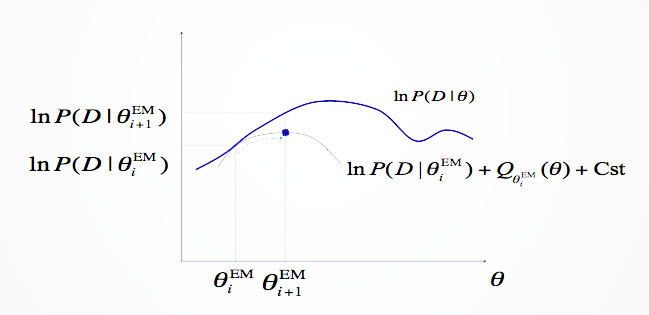
\includegraphics[width=.8\linewidth]{figs/EMcurve.png}}
\caption{Search for the optimum $\theta$ using the Expectation-Maximization Algorithm.}\label{fig:emcurve}
\end{figure}

The algorithm works as follows: \textcolor{red}{ok or not ???}
\begin{itemize}
\item Given: $D$
\item Initialization: set $i=0$; set $\theta_0^{EM}$ to an initial guess
\item Repeat until $\delta \approx 0$:

Expectation step: compute $Q_{\theta_i^{EM}}(\theta)$ using eq. (\ref{eq:QEM}) and the parameters $\theta_{i}^{EM}$ from the previous iteration.

Maximization step: compute $\theta_{i+1}^{EM}$ by maximizing $Q_{\theta_i^{EM}}(\theta)$ as shown in eq. (\ref{eq:thetaEM})

Update $\delta$ using eq. (\ref{eq:deltaEM})

$i = i + 1$

\item Output $\theta_i^{EM}$
\end{itemize}

\subsection{Baum-Welch algorithm}

The Baum-Welch algorithm is a special case of EM where:\\
$D=x$, $m=\pi$, and $\theta = \{ \{ a_kl \}, \{ e_k(b) \} \}$.

\subsection{Motif finding}

context: transcription regulation for the expression of genes

enhancer and silencer regions: sites where prots bind, right combination of prots bring RNA pol together or block it to start transcribing the gene

multiple co-regulated genes have a similar TF binding site

simplification: Each DNA sequence contains only one copy of the TF binding site. the motif has fixed length (given).

motif = binding site (not exact match)

motif finding: find the position of the motif in each sequence, without knowing how the motif looks like: we only know that it occurs only once. so the problem is to find the best common motif shared among all sequences (like a local alignment but for multiple sequences)

Prob of seq given the position $Prob(S|a,\theta_W, \theta_0)$

\begin{equation}
\ln \; P(s_k|a_k,\theta) = \sum_{i=1}^{a_k-1} \ln \; \theta_{b_i^k}^0
                  + \sum_{i=1}^w \ln \; \theta_{b_{a_k + i - 1}^k}^i
                  + \sum_{i=a_k+w}^{L_k} \ln \; \theta_{b_i^k}^0
\end{equation}
for simplification assume that all positions have the same probability of containing the motif:
\begin{equation}
P(a_k | \theta) = \frac{1}{L_k}
\end{equation}

path has only one degree of freedom: at which position you enter the motif part.
similar to running viterbi and getting best path.
but here no dyn progr because only one degree of freedom, so no need for dyn progr: basically just need to locate motif: best position in seq:

repeat this process: get motif, score in seq, get best pos, look at this pos, create new motif, repeat, guaranteed to converge like viterbi, but very greedy, so might converge to poor solution.

can run EM on this, but now no need to run fwd and backw algorithm, because only one degree of freedom

termination: convergence of the alignment and the motif matrix

then missing variables n here are the starting positions of the motif in each seq

sum_m = 
sum over all possible configs of missing variables m:
instead of all possible configs (too many, combinatorial), use:
sum_n sum_m_n: for all seqs, sum over all possible positions of the motif in seq

...

this is the core of expectation maximization:
in EM we say:
there are missing (hidden) variables:
given current parameters we can score all possible configs of missing variables, to each of these configs we assign a probability, 
take all possible configs of missing variables and let them contribute to the update of parameters but according to their probability
- don't take best guess: take all possible guesses, weighted by their probs: bad guesses weight very little, good guesses weight higher

difference between viterbi and EM:
in both there are missing (hidden) variables:
- in viterbi we score the possible configs of missing vars, and select best config based on current parameters, select this best to construct next model
- take the best guess for missing variables to update

%---------------------------------------------------------------------------

